\begin{figure}[t]
  \hspace{0.05\textwidth}%
  \begin{subfigure}[b]{\textwidth}
    \tikzstyle{legend-point}=[circle, inner sep=2pt]
    \definecolor{legend1}{HTML}{4c72b0}
    \definecolor{legend2}{HTML}{55a868}
    \definecolor{legend3}{HTML}{c44e52}
    \definecolor{legend4}{HTML}{8172b2}
    \definecolor{legend5}{HTML}{ccb974}
    
    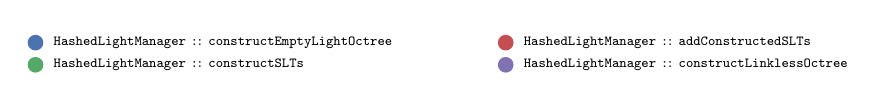
\begin{tikzpicture}
      \node (legend1) at (0.1\textwidth, 0)
            [legend-point, fill={legend1}, label=right:{\tiny $\mathtt{HashedLightManager::constructEmptyLightOctree}$}] {};
      \node (legend2) at (0.1\textwidth, -8pt)
            [legend-point, fill={legend2}, label=right:{\tiny $\mathtt{HashedLightManager::constructSLTs}$}] {};
      \node (legend6) at (0.5925\textwidth, 0)
            [legend-point, fill={legend3}, label=right:{\tiny $\mathtt{HashedLightManager::addConstructedSLTs}$}] {};
      \node (legend7) at (0.5925\textwidth, -8pt)
            [legend-point, fill={legend4}, label=right:{\tiny $\mathtt{HashedLightManager::constructLinklessOctree}$}] {};
    \end{tikzpicture}
  \end{subfigure}\hfill\\
  \begin{adjustbox}{minipage=\textwidth, scale=0.55}
    \begin{subfigure}[b]{0.8\textwidth}
      \centering
      \def\svgwidth{\textwidth}
      \input{./img/raw/hs-layered-exec/layered_spaceship-indoor_70.pdf_tex}
      \caption{Spaceship Indoor - 70 lichten}
      \vspace{4pt}
      \label{fig:hs-layered-exec:indoor-70}
    \end{subfigure}
  \end{adjustbox} %
  %
  \begin{adjustbox}{minipage=\textwidth, scale=0.55}
    \begin{subfigure}[b]{0.8\textwidth}
      \centering
      \def\svgwidth{\textwidth}
      \input{./img/raw/hs-layered-exec/layered_spaceship-indoor_1260.pdf_tex}
      \caption{Spaceship Indoor - 1260 lichten}
      \vspace{4pt}
      \label{fig:hs-layered-exec:indoor-1260}
    \end{subfigure}
  \end{adjustbox} \\
  %
  \begin{adjustbox}{minipage=\textwidth, scale=0.55}
    \begin{subfigure}[b]{0.8\textwidth}
      \centering
      \def\svgwidth{\textwidth}
      \input{./img/raw/hs-layered-exec/layered_pipers-alley_58.pdf_tex}
      \caption{Piper's Alley - 58 lichten}
      \label{fig:hs-layered-exec:alley-58}
    \end{subfigure}
  \end{adjustbox}
  %
  \begin{adjustbox}{minipage=\textwidth, scale=0.55}
    \begin{subfigure}[b]{0.8\textwidth}
      \centering
      \def\svgwidth{\textwidth}
      \input{./img/raw/hs-layered-exec/layered_pipers-alley_1044.pdf_tex}
      \caption{Piper's Alley - 1044 lichten}
      \label{fig:hs-layered-exec:alley-1044}
    \end{subfigure}
  \end{adjustbox} \\
  %
  \begin{adjustbox}{minipage=\textwidth, scale=0.55}
    \begin{subfigure}[b]{0.8\textwidth}
      \centering
      \def\svgwidth{\textwidth}
      \input{./img/raw/hs-layered-exec/layered_ziggurat-city_65.pdf_tex}
      \caption{Ziggurat City - 65 lichten}
      \label{fig:hs-layered-exec:city-65}
    \end{subfigure}
  \end{adjustbox} %
  %
  \begin{adjustbox}{minipage=\textwidth, scale=0.55}
    \begin{subfigure}[b]{0.8\textwidth}
      \centering
      \def\svgwidth{\textwidth}
      \input{./img/raw/hs-layered-exec/layered_ziggurat-city_1170.pdf_tex}
      \caption{Ziggurat city - 1170 lichten}
      \label{fig:hs-layered-exec:city-1170}
    \end{subfigure}
  \end{adjustbox}
  \caption{\small Constructietijd per stap als functie van de knoopgrootte.}
  \label{fig:hs-layered-exec}
\end{figure}
